
\subsection{Results}

\subsubsection{Post Test Check}

The post-test data make it possible to ensure that participants
possessed the appropriate structured knowledge for each trial.
For instance, if participants did not realise that
dolphins and llamas belong to the same biological group (mammals)
then we cannot asses the interaction of
associative and structured knowledge when reasoning about these species.
Appendix~\ref{appendix:exp3_posttest} shows the proportion of participants
who correctly identified that the base and correct response species
belonged to the same taxonomic group,
and that the base and foil response species did not,
for the stimuli used in the experimental trials.
Participants only performed above chance on the post-test
for the correct response species for 7 of the 14 stimuli sets
(binomial test, N=40, 67.5\% accuracy required for p < .05),
and so only these sets were included in the subsequent analyses.

  
\subsubsection{Reasoning Accuracy}

Due to an error in the software used to run the experiment,
mouse cursor data were recorded incorrectly on 40 trials (7.1\% of total)
in which participants took more than 2,200 msec to respond,
and so these trials were discarded from the analysis.
In the analyses that follow, I fitted linear or logistic mixed models, 
with random intercepts for each participant, and for each stimulus set.

Participants were significantly more likely to
choose the foil species on conflict trials,
where the foil and the base were strongly associated (26\%),
than on control trials, where they were not (5\%;
$e^{\beta}$ = 10.6, CI = [5.2; 21.8],
z = 6.421, p < .0001).
It may be the case that this effect is driven by
a subset of participants who are influenced by associative knowledge.
Figure~\ref{fig:exp3_acc} shows each participant's number of foil responses, by condition.
Of the 40 participants, 30 gave the foil response more often under conflict,
none did so more often on control trials,
and 10 never gave the foil response.
Therefore, the main effect on participants' responses
appears to apply across all participants,
or at least all participants who did not achieve perfect accuracy.

\begin{figure}[ht]
  \centering
  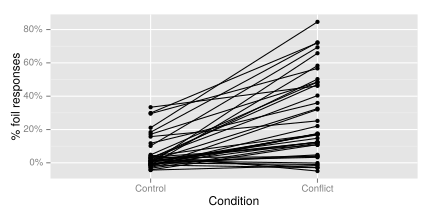
\includegraphics[width=\figurewidth]{imgs/exp3_acc.pdf}
  \caption[Participants' number of foil responses, by condition, Experiment 3.]{
    \label{fig:exp3_acc}
    Participants' number of foil responses, by condition.
    Of 40 participants, 30 gave more foil responses under conflict,
    and 10 never gave the foil response.
}
\end{figure}



\subsubsection{Correct Responses}

On trials in which the correct response was given,
there was no difference in response time between the conditions
(1,264 msec in conflict condition, SD = 297,
1,273 msec in control condition, SD = 361; t < .8, p > .4).
Participants were significantly faster to initiate the mouse movements
for correct responses in the conflict condition (628  msec, SD = 213)
than in the control condition (688 msec, SD = 206;
$e^{\beta}$ = 89\%, CI = [84\%, 95\%], t(405.2) = 3.670, p < .0001).

Maximum Deviation was bimodally distributed
(Bimodality Coefficient = .705; Hartigan's D = .0422, N = 520, p < .0001),
and trajectories were classified as either
direct trajectories or reversals, as described in Chapter 2 (MD cut-off = 0.524).
A significantly greater proportion of
trials where participants selected the correct species
were classed as reversals
in the conflict condition (16\%)
than the control condition (8\%;
$e^{\beta}$ = 2.2, CI = [1.2; 3.9], z = 2.524, p = .0116).
Therefore, although response latencies do not suggest conflict,
analysis of participants' mouse cursor movements shows that
responses based on structured knowledge
showed a greater attraction towards the foil response option
when the foil was strongly associated with the base species.

\subsubsection{Cursor Trajectories}

Once again, cursor trajectories in this experiment
can be classed as either
Direct Correct, Reversal Correct, Reversal Foil, or Direct Foil trajectories.
Table~\ref{tbl:exp3_trajectories} shows the proportion of
each trajectory type by condition.
Under conflict, there was a small increase in the number of
Reversal Correct responses,
and a considerably larger increase in the number of incorrect responses.

\begin{table}[h]
  \centering
    \caption[Kinds of trajectory in Experiment 3.]{
    \label{tbl:exp3_trajectories}
    Proportion of each trajectory type, by condition.
    Under conflict, participants were markedly more likely to 
    directly move to the foil option,
    and less likely to directly move to the correct option.
  }
  \begin{tabular}{lrrrr}
    \toprule
             & Direct Correct & Reversal Correct & Reversal Foil & Direct Foil\\
    \midrule
    Control  & 87\%           & 8\%              & 0.8\%         & 4\%\\
    Conflict & 62\%           & 12\%             & 3\%           & 23\%\\
    \bottomrule
  \end{tabular}
\end{table}


% |     &nbsp;     |   a   |   b    |   c    |
% |:--------------:|:-----:|:------:|:------:|
% |  **control**   | 88.2% | 99.09% | 32.2%  |
% |  **conflict**  | 64.7% | 95.83% | 66.01% |

Transition probabilities for trajectories from this experiment
are shown in Table~\ref{tab:exp3_transitions_table}.
Participants were significantly more likely to 
initially move towards the correct species on control trials (88\%)
than conflict trials (65\%;
$e^{\beta}$ = 4.7, CI = [2.9; 7.6], z = 6.284, p < .0001).
On trials where they have moved towards the correct option,
participants were also more likely to select it
on control trials (99\%) than conflict trials (96\%;
$e^{\beta}$ = 5.2, CI = [1.04; 26.2], z = 2.006, p = .0448),
although in both cases participants who initially move towards the correct option
are extremely unlikely to subsequently change direction.
Finally, on the trials where participants did initially move towards the foil option,
they are more likely to change direction
and select the correct option instead
on control trials (68\%)
than on conflict trials (34\%;
$e^{\beta}$ = 16.9, CI = [3.6, 80.2], z = 3.567, p = .0004).

Lastly, on conflict trials, movement initiation times
did not differ significantly between
initial movements that were towards the correct option (617 msec, SD = 225)
and those towards the foil option (652 msec, SD = 201;
t(251.8) = 1.365, p = .1733).

\begin{figure}[ht]
  \begin{floatrow}
    \ffigbox[.5\textwidth]{%
    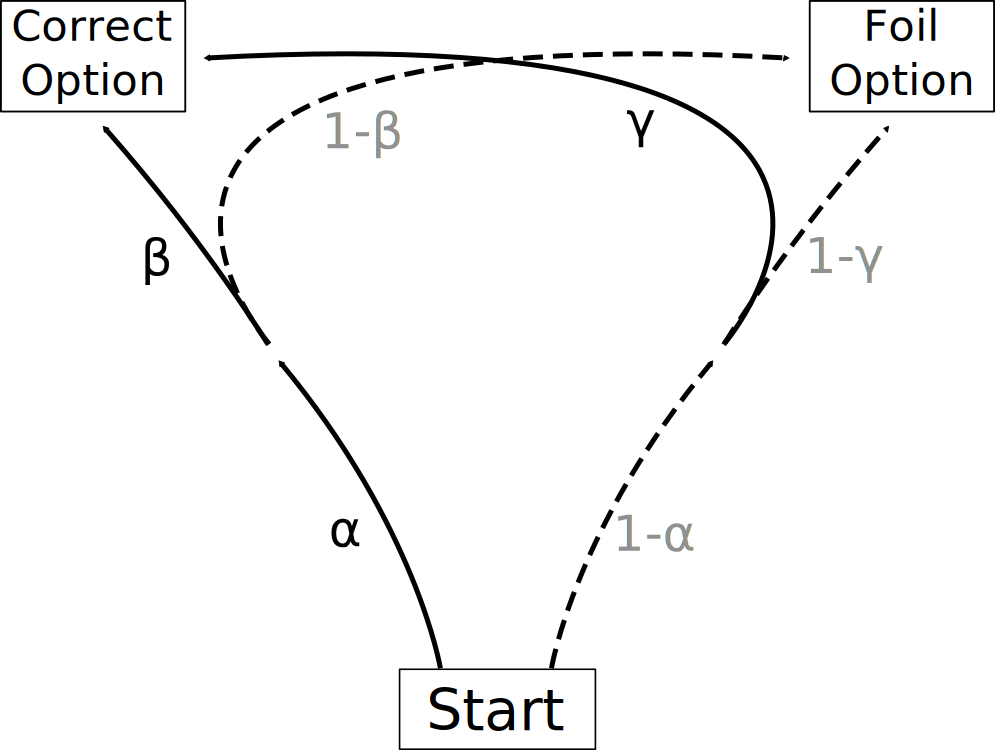
\includegraphics[width=.5\textwidth]{../2.Methods/imgs/transitions.pdf}
    }{%
      \caption[The possible transitions that can occur during a trial.]{
        The possible transitions that can occur during a trial.
        \label{fig:exp3_transitions}
    }
    }
    \capbtabbox{%
      \centering
      \begin{tabular}{lPP}
        \toprule
        Parameter & Control & Conflict  \\
        \midrule
        $\alpha$  & 88\%    & 65\%^{***} \\ % p = 3.28e-10
        $\beta$   & 99\%    & 96\%^{*}   \\ % p = .044
        $\gamma$  & 68\%    & 34\%^{***} \\ % p = 0.00036
        \bottomrule
        \multicolumn{3}{l}{
          \emph{Note}: $^{*} p < .05;\ ^{**}p < .01;\ ^{***} p < .001.$
        }
      \end{tabular}
      %% \begin{tabular}{cc} \hline
      %%   Author & Title \\ \hline
      %%   Knuth & The \TeX book \      Lamport & \LaTeX \\ \hline
      %% \end{tabular}
    }{%
      \caption{
        Transition probabilities for Experiment~3.
        \label{tab:exp3_transitions_table}
      }%
    }
  \end{floatrow}
\end{figure}


\subsubsection{Time Course}

Figure~\ref{fig:exp3_condition_timecourse} plots
the proportion of trials in which the cursor is on
the foil species' side of the screen (top),
and the correct species' side (bottom),
broken down by condition.
For each plot, a series of logistic mixed models were fit,
with the probability of the cursor being on
that side of the screen predicted by condition (control or conflict),
across each 20 msec window, from 100 to 1,000 msec.
Random intercepts were included for each participant and for each base species.
By identifying the points from which
there were significant effects of condition in each series of models,
we can see at what point in time
manipulating the association of the foil species
affected participants' cursor trajectories
to that side of the screen.
Trials in the conflict condition were more likely to move towards
the foil response than those in the control condition from 480 msec onwards.
Those in the control condition were more likely to move towards
the correct response than those in the conflict condition from 760 msec onwards.

Figure~\ref{fig:exp3_side_timecourse} shows the same data,
but with separate plots for the control (top) and conflict (bottom) conditions,
and separate lines corresponding to the proportion of trials
on each side of the screen.
Divergence times were calculated in the same way,
this time reflecting the point, in each condition,
that participants became more likely to move towards
the correct species than the foil.
In both conditions, this divergence occurred at 480 msec.
This means that while participants selected the foil option
significantly more often on conflict trials than control trials,
they were no slower to show a preference for the correct species under conflict.

\begin{figure}[tp]
  \centering
  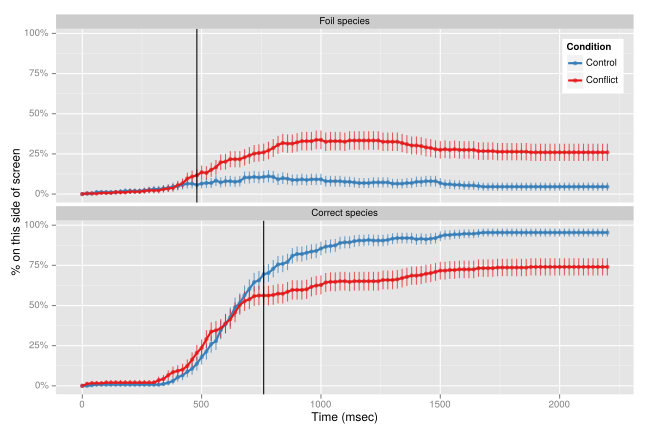
\includegraphics[width=.9\textwidth]{imgs/exp3_condition_timecourse.pdf}
  \caption[Time course, seperately for each condition, Experiment 3.]{
    Proportion of trials on each half of the screen, over time.
    Vertical lines show the points from which
    there were significant differences between
    the control and conflict conditions.
    \label{fig:exp3_condition_timecourse} }
\end{figure}

\begin{figure}[bp]
  \centering
  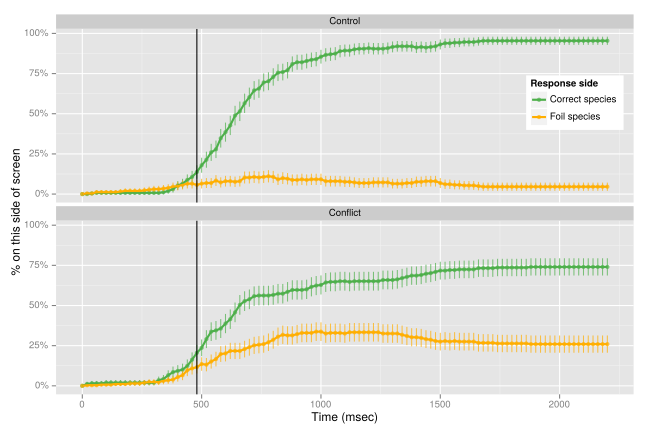
\includegraphics[width=.9\textwidth]{imgs/exp3_side_timecourse.pdf}
  \caption[Time course, seperately for each response option, Experiment 3.]{
    Proportion of cursors on each half of the screen, over time.
    Vertical lines show point from which participants were
    more likely to move towards the correct option
    than the foil.
    \label{fig:exp3_side_timecourse} }
\end{figure}

Recall that in Experiments 1 and 2,
the plots corresponding to the bottom panel of Figure~\ref{fig:exp3_side_timecourse}
showed a cross-over trend:
participants were initially more likely to move towards the foil option,
with this initial preference fading, and eventually reversing,
as the correct option was chosen on the majority of trials.
Here, instead, we see that participants 
are never more likely to move towards the foil option than the correct one.
The implications of these temporal dynamics are discussed below.

